\chapter{Súčasný stav VST syntetizátorov}
\label{sucasnystav}

Pre potreby návrhu a implementácie akéhokoľvek druhu softvéru je nevyhnutné pochopiť princípy jeho fungovania, osvojiť si zvyky a štandardy, zaužívané v aplikáciách tohto typu, zistiť nevýhody a chyby v existujúcich implementáciách a tiež nechať sa inšpirovať zaujímavými a užitočnými prvkami týchto implementácií. Je veľmi užitočné urobiť prieskum medzi odborníkmi pracujúcimi v danej oblasti, ktorí sa každodenne s daným typom softvéru stretávajú, čo im na existujúcom softvéri vyhovuje, čo im prekáža a čo im chýba. Toto isté platí aj pre vytváranie softvérového syntetizátora.

\section{Ponuka voľne šíriteľných VST syntetizátorov}

V súčasnosti je k dispozícii veľké množstvo rôznych druhov VST syntetizátorov a aj niekoľko internetových stránok ponúkajúcich databázy existujúcich produktov. Najvýznamnejšou z týchto stránok je stránka \emph{KVR~AUDIO} (kvraudio.com), ktorá ponúka komplexný prehľad o existujúcich nástrojoch a efektoch, tak komerčných, ako aj voľne šíriteľných, a ponúka aj mnohé iné služby pre vývojárov aj pre samotných používateľov. Na stránke KVR AUDIO je možné vyhľadávanie v databáze podľa mnohých kritérií.

Témou tejto práce je navrhnúť a implementovať subraktívny syntetizátor. Na účely zhodnotenia stavu subtraktívnych nástrojov pre rozhranie VST som vybral skupinu voľne šíriteľných syntetizátorov, pretože komerčné nástroje sú často komplexné, kombinujúce rôzne druhy syntéz, a navyše nie všetky ponúkajú plne funkčnú demoverziu. Na webstránke KVR AUDIO som pri vyhľadávaní vybral kategóriu freeware subtraktívnych syntetizátorov pre rozhranie VST kompatibilné s operačným systémom Windows XP. Z 235 nájdených výsledkov som rýchlym testovaním vyradzoval tie, ktoré hneď v prvých minútach testovania pôsobili neseriózne, neprístupne a nestabilne. Týmto testom prešlo úspešne len vyše 60 syntetizátorov, z ktorých som hlbším testovaním vybral 30 najlepších. Keďže nemám so syntetizátormi zďaleka toľko skúseností, ako tvorcovia hudby, požiadal som štyroch elektronicky zameraných hudobníkov z komunity \emph{Corenforce} o pomoc pri testovaní.

\section{Kritériá testovania}

Najdôležitejšími kritériami pri testovaní boli:

\begin{description}
\setlength{\itemsep}{-0.5ex}
\item[Kvalita zvuku] -- harmonický obsah, ruchy, aliasy, kvalita filtrov a efektov,
\item[Rozsiahlosť možností] -- či je syntetizátor schopný vytvoriť široké spektrum rôznych zvukov,
\item[Ovládanie a intuitívnosť] -- či syntetizátor reaguje predvídateľne a správne na používateľské vstupy,
\item[GUI a prehľadnosť] -- kvalita používateľského rozhrania, logická štruktúra a rozmiestnenie komponentov.
\end{description}

Od hudobníkov som požadoval krátke zhrnutie pozitívnych a negatívnych stránok každého syntetizátora, a celkové hodnotenie použitím stupnice 0 -- 10 bodov.

\section{Vyhodnotenie výsledkov testu}


\begin{table}[h]
\centering
\begin{tabular}{|r|l|l|}
\hline
umiestnenie & názov (výrobca) & priemerné hodnotenie\\
\hline \hline
1. & \textbf{Superwave P8} (Superwave) & 7,8\\
\hline 
2. & \textbf{Syncaine TM-200X} (Syncer) & 7,5\\
 & \textbf{SubDuer} (Majken) & 7,5\\
\hline 
4. & \textbf{Evol} (Synthtronic) & 6,9\\
\hline 
5. & \textbf{Lallapallooza} (Buzzroom) & 6,8\\
\hline
\end{tabular}
\caption{Výsledok hodnotenia syntetizátorov hudobníkmi}
\label{tab01}
\end{table}
\vspace{10 mm}


\begin{figure}[h]%
\centering
\centering
\resizebox{10cm}{!}{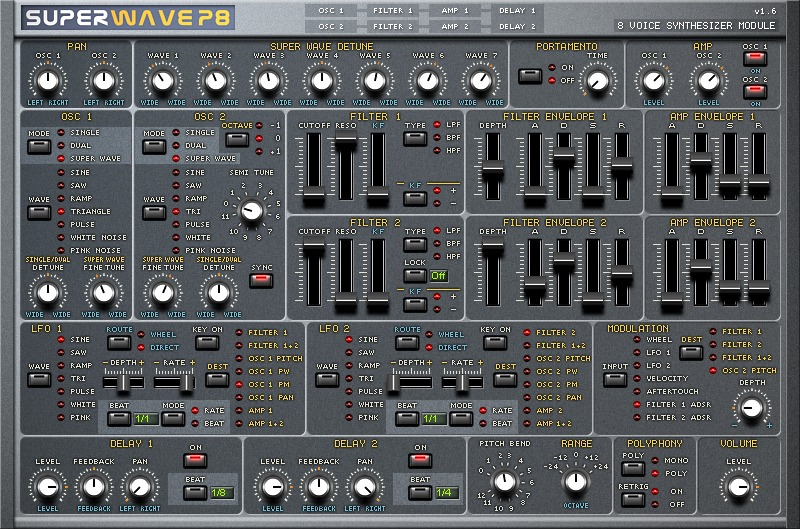
\includegraphics{p8.jpg}}\\
Superwave P8
\end{figure}
\vspace{10 mm}

\begin{figure}[h]%
\centering
\begin{minipage}[h]{7cm}
\centering
\resizebox{7cm}{!}{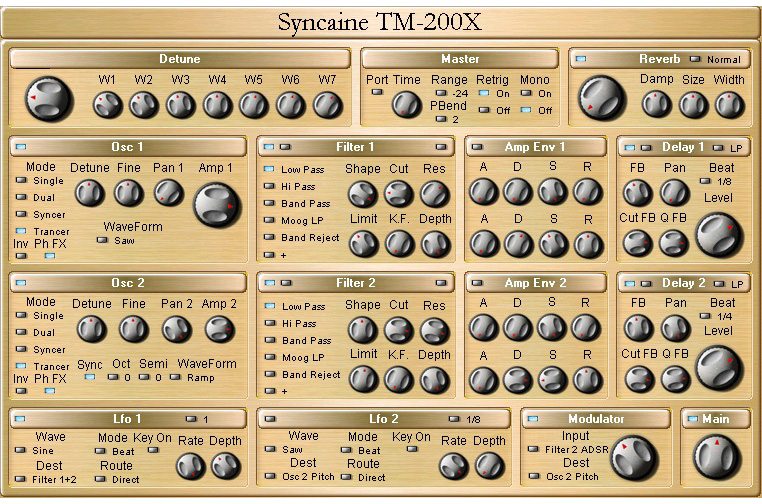
\includegraphics{syncaine.jpg}}
Syncaine TM-200X
\end{minipage}
\quad
\begin{minipage}[h]{7cm}
\centering
\resizebox{7cm}{!}{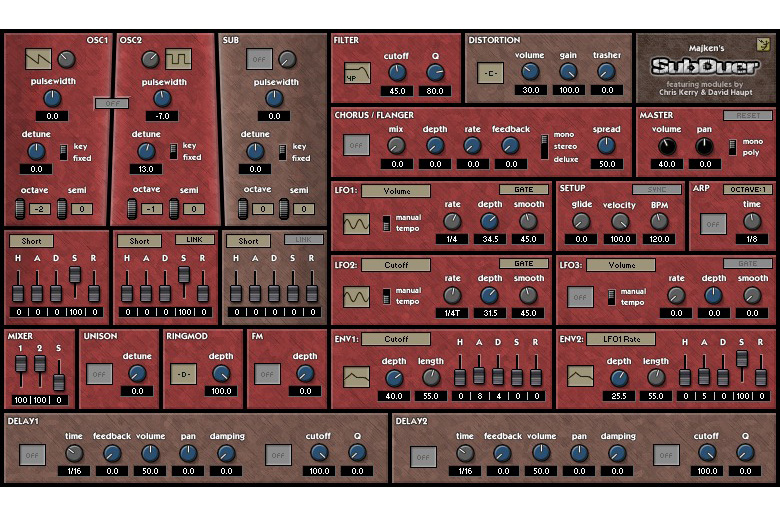
\includegraphics{subduer.jpg}}
SubDuer
\end{minipage}
\vspace{5 mm}
\caption{Prvé tri najlepšie subtraktívne syntetizátory}
\label{obr05}
\end{figure}%
\vspace{5 mm}
\noindent
Bodové hodnotenia syntetizátorov od jednotlivých hudobníkov boli celkom podobné, čo naznačuje určitú mieru objektivity výsledkov testovania. Priemerná odchýlka hodnotenia konkrétneho syntetizátora hudobníkom od priemeru jeho hodnotení je 1,2 bodu. Päť najlepšie ohodnotených syntetizátorov je uvedených v tabuľke \ref{tab01}. Bodové hodnotenia sami o sebe nenesú hodnotnú informáciu o konkrétnych výhodách alebo chybách a nedostatkoch jednotlivých syntetizátorov užitočných pre návrh nového nástroja. Z tohto dôvodu som vyžadoval od testujúcich hudobníkov aj krátky textový popis zdôvodňujúci hodnotenie. 

\subsection{Chyby a nedostatky testovaných syntetizátorov}

Pri porovnávacích testoch vyplávalo na povrch mnoho chýb a nedostatkov. Tie významné nedostatky beriem do úvahy pri návrhu vlastného syntetizátora.

\subsection*{Chyby vo zvukovom výstupe}

\begin{description}
\setlength{\itemsep}{-0.5ex}
\item[Falošné tóny] -- nepresné prepočty frekvencií zodpovedajúcich konkrétnym notám spôsobujú počuteľné rozladenie vysokých a nízkych oktáv.
\item[Pískanie rezonancie filtra] -- rezonančné pásmo filtra je príliš úzke a namiesto príjemného zvýraznenia hraničného pásma vzniká nepríjemné pískanie. Touto chybou trpí veľká skupina testovaných syntetizátorov, zrejme z dôvodu použitia toho istého filtrovacieho algoritmu.
\item[Iné nedostatky filtra] -- málo druhov filtra, napríklad len lowpass, nežiaduce efekty pri zmene parametrov.
\end{description}

\subsection*{Chyby v ovládaní}

\begin{description}
\setlength{\itemsep}{-0.5ex}
\item[Neštandardný systém točenia potenciometrov] -- nástroj ignoruje nastavenie hos\-tu o systéme točenia potenciometrov, prehnaná citlivosť parametrov, pri ktorej je obtiažne trafiť konkrétnu hodnotu.
\item[Neštandardné fungovanie komponentov] -- ovládanie nástroja nezodpovedá zaužívaným spôsobom fungovania syntetizátorov a pri takomto nedostatku nie je možné s nástrojom intuitívne pracovať.
\item[Absencia zobrazovania hodnôt parametra] -- bez zobrazovania hodnoty parametra nemožno nastaviť požadované hodnoty presne.
\item[Malý rozsah parametra] -- nemožnosť nastaviť určité hodnoty, napríklad lowpass filter pri maximálnej hodnote hraničnej frekvencie neprepúšťa celé počuteľné spektrum, ale počuteľne filtruje vysoké frekvencie. 
\item[Pukanie pri točení parametrov] -- pri rýchlom točení parametrov sa hodnoty menia nespojito, čo pri viacerých parametroch vytvára nežiaduce vysokofrekvenčné impulzy. 
\end{description}

\subsection*{Ostatné chyby}

\begin{description}
\setlength{\itemsep}{-0.5ex}
\item[Neestetický dizajn] -- veľmi negatívne ovplyvňuje prácu s nástrojom.
\item[Nelogické alebo neprehľadné rozmiestnenie ovládacích prvkov] -- \hspace{1 mm} nie je možné intuitívne meniť požadované parametre, slabý kontrast ovládacích prvkov oproti pozadiu.
\item[Zbytočne veľká plocha syntetizátora] -- pracovná plocha monitora je veľmi drahá a syntetizátory využívajúce túto plochu neefektívne značne znižujú produktivitu práce.
\item[Nečitateľnosť] -- použitie neštandardných skratiek s cieľom ušetriť plochu vedie k nejasnosti, čo ktorý parameter ovláda.
\item[Nestabilita] -- pri určitých nastaveniach syntetizátor prestane vydávať zvuk a je nutné ho reštartovať.
\item[Absencia podpory rôznych vzorkovacích frekvencií] -- neberie do úvahy vzorkovaciu frekvenciu a generuje zvuk vždy konštantne vzhľadom na vzorky alebo po zmene vzorkovacej frekvencie prestáva fungovať úplne.
\end{description}

\subsection{Výhody testovaných syntetizátorov}

Niektoré syntetizátory vynikali oproti iným určitými ojedinelými vlastnosťami, ktoré buď rozširovali možnosti použitia syntetizátora, alebo uľahčovali prácu s ním.

\begin{description}
\setlength{\itemsep}{-0.5ex}

\item[Neštandardné priebehy oscilátorov] -- ponúkajú iné spektrá zvukov ako bežne používané priebehy.
\item[Rozsiahle modulačné možnosti] -- čím viac je možností modulácie, tým menej obmedzené je spektrum zvukov a zvukových efektov, ktoré je možné vygenerovať.
\item[Viac ako jeden filter] -- viac filtrov s možnosťou rôzneho vzájomného zapojenia prináša nielen väčšiu kontrolu nad frekvenčným spektrom zvuku, ale aj väčšiu variabilitu strmosti filtrovania.
\item[Rôzne strmosti filtrov] -- bežne používané 12, 18 a 24 dB/oct.
\item[Unisono] -- pridanie jedného alebo viacerých mierne rozladených oscilátorov pre generovanie mohutnejšieho zvuku.
\item[Integrované efekty] -- chorus, delay, reverb, phaser alebo iné efekty pre spestrenie zvukových možností.
\item[Nadštandardné obálky] -- čo najväčšia kontrola nad vývinom zvuku v čase.
\item[Graficky znázornené parametre] -- pre čo najväčšiu prehľadnosť a intuitívnosť.

\end{description}

